\chapter{\LaTeX{}使用说明}\label{chap:guide}

为方便使用及更好地展示\LaTeX{}排版的优秀特性,cuzthesis对框架和文件体系进行了细
致地处理,尽可能地对各个功能和板块进行了模块化和封装,对于初学者来说,众多的文件
目录也许一开始让人觉得有些无所适从,但阅读完下面的使用说明后,会发现原来使用思路
是简单而清晰的;而且,当对\LaTeX{}有一定的认识和了解后,会发现其相对Word类排版系
统极具吸引力的优秀特性。故若是初学者,请不要退缩,请稍加尝试和坚持,以领略到
\LaTeX{}的非凡魅力,并可以通过阅读相关资料如\LaTeX{}
Wikibook\citep{wikibook2014latex}来完善自己的使用知识。

\section{新手上路}

\begin{enumerate}
    \item 安装软件:根据所用操作系统和章节~\ref{sec:system}中的信息安装\LaTeX{}
    编译环境。
    \item 获取模板:下载 \href{https://github.com/xiehao/CUZThesis}{cuzthesis}
    模板并解压。cuzthesis模板不仅提供了相应的类文件,同时也提供了包括参考文献等
    在内的完成学位论文的一切要素,所以,下载时,推荐下载整个cuzthesis文件夹,而
    不是单独的文档类。
    \item 编译模板:
        \begin{enumerate}
            \item Windows:双击运行artratex.bat脚本。
            \item Linux或macOS: {\small \verb|terminal| -> \verb|chmod +x ./artratex.sh| -> \verb|./artratex.sh xa|}
            \item 任意系统:都可使用\LaTeX{}编辑器打开cuzthesis.tex文件并选择
            \hologo{XeLaTeX}编译引擎进行编译。
        \end{enumerate}
    \item 错误处理:若编译中遇到了问题,请先查看“常见问题”(章节
    ~\ref{sec:qa})。
\end{enumerate}

编译完成即可获得本PDF说明文档,而这也完成了学习使用cuzthesis撰写论文的一半进程。
至此,新手已上路!

\section{文档目录简介}

本部分主要介绍cuzthesis工程的目录结构,以助读者理解各部分含义。

\subsection{cuzthesis.tex}

cuzthesis.tex为主文档,其设计和规划了论文的整体框架,通过对其的阅读可以了解整个
论文框架的搭建。如无意外,读者无需修改此文档。

\subsection{编译脚本}

\begin{itemize}
    \item Windows:双击批处理文件artratex.bat可得全编译后的PDF文档,其存在是为了
    帮助不了解\LaTeX{}编译过程的初学者跨过编译这第一道坎,请勿通过邮件传播和接收
    此脚本,以防范DOS脚本的潜在风险。
    \item Linux或macOS:在终端中运行
        \begin{itemize}
            \item \verb|./artratex.sh xa|:获得全编译后的PDF文档
            \item \verb|./artratex.sh x|:快速编译模式
        \end{itemize}
    \item 全编译指运行 \verb|xelatex+bibtex+xelatex+xelatex| 以正确生成所有的引
    用链接,如目录,参考文献及引用等。在写作过程中若无添加新的引用,则可用快速编
    译,即只运行一遍\LaTeX{}编译引擎以减少编译时间。
\end{itemize}

\subsection{cache文件夹}

运行上述编译脚本后,编译所生成的中间文件与最终PDF文档皆存于该文件夹内,其存在是
为了保持工作空间的整洁,因为好的心情是很重要的。若自行编译(即不运行上述编译脚
本)则不在该文件夹下生成文件。

\subsection{styles文件夹}

该文件夹包含cuzthesis文档类的定义文件和配置文件,通过对它们的修改可以实现特定的
模版设定。若需更新模板,一般只需用新的样式文件替换旧的即可。该部分为模板编写者修
改之用,一般读者亦无需修改此部分。

\begin{enumerate}
    \item cuzthesis.cls:文档类定义文件,论文的最核心的格式即通过它来定义的。
    \item cuzthesis.cfg:文档类配置文件,为类定义文件准备常量标签等配置信息。
    \item artratex.sty: 常用宏包及文档设定,如参考文献样式、文献引用样式、页眉页
    脚设定等。这些功能具有开关选项,常只需在thesis.tex中的如下命令中进行启用即
    可,一般无需修改artratex.sty本身。
        
        \path{\usepackage[options]{artratex}} 
    \item artracom.sty:自定义命令以及添加宏包的推荐放置位置。
\end{enumerate}

\subsection{contents文件夹}

该文件夹内为论文的所有实体内容,正常情况下,这也是\textbf{使用cuzthesis撰写学文
论文时,主要关注和修改的一个位置。注:所有文件都必须采用UTF-8编码,否则编译后将
出现乱码文本},详细介绍如下:

\begin{itemize}
    \item initialization.tex:为论文中出现的一些必要信息的初始化,如:中英文标
    题、作者名、学号、专业、学院、毕业年份等等,这些信息变量一旦设置一次之后,后
    面很多地方即可直接调用。
    \item mainbody.tex:索引需要出现的章节。开始写论文时,可以只索引当前章节,以
    快速编译查看,当论文完成后,再对所有章节进行索引即可。
    \item abstracts.tex:中英文摘要的内容。
    \item chapter{\_}xxx.tex:为论文主体的各个章节,即mainbody.tex文件中索引的章
    节,可根据需要添加和撰写(建议将xxx替换为相应章节的全小写英文名,如
    introduction等)。
    \item acknowledgement.tex:致谢的内容。
    \item appendices.tex:为附录内容,如无此部分可将其在cuzthesis.tex文件中的导
    入语句注释掉
\end{itemize}

\subsection{images文件夹}

该文件夹用于放置论文中所需要的图片类文件,支持格式有:.jpg, .png, .pdf。其中,
cuz{\_}logo.pdf为浙传校徽文件,用于创建封面。建议将清晰的矢量图(如流程图、框架
图、模块图等)转换成.pdf格式并裁剪到合适大小,而位图则以.png格式为佳。原则上,能
用矢量图的尽量不要用位图。此外,不建议为各章节图片建子目录,即使图片众多,若命名
规则合理,图片查询亦是十分方便。

\subsection{bibliography文件夹}

该文件夹主要用于存放参考文件格式定义文件与内容信息,

\begin{enumerate}
    \item references.bib:参考文献内容信息库。
    \item gbt7714-xxx.bst:符合国标的文献样式定义文件。由
    \href{https://github.com/zepinglee/gbt7714-bibtex-style}{zepinglee}开发,并
    满足最新国标要求。与文献样式有关的问题,请查阅开发者所提供的文档,并建议适当
    追踪其更新。
\end{enumerate}

\section{排版元素}

学位论文中的排版元素有很多,本模板无法逐一介绍,只就公式、图表等几种常用的排版元
素的用法及注意事项简要说明如下,详细用法请参考相应资料。

\subsection{数学公式}

比如Navier-Stokes方程,如式\eqref{eq:ns}和式\eqref{eq:ns-}所示:
\begin{equation}
    \label{eq:ns}
    \begin{cases}
        \frac{\partial \rho}{\partial t} + \nabla\cdot(\rho\Vector{V}) = 0 \ \mathrm{times\ font\ test}\\
        \frac{\partial (\rho\Vector{V})}{\partial t} + \nabla\cdot(\rho\Vector{V}\Vector{V}) = \nabla\cdot\Tensor{\sigma} \ \text{times font test}\\
        \frac{\partial (\rho E)}{\partial t} + \nabla\cdot(\rho E\Vector{V}) = \nabla\cdot(k\nabla T) + \nabla\cdot(\Tensor{\sigma}\cdot\Vector{V})
    \end{cases}
\end{equation}
\begin{equation}
    \label{eq:ns-}
    \frac{\partial }{\partial t}\int\limits_{\Omega} u \, \mathrm{d}\Omega + \int\limits_{S} \unitVector{n}\cdot(u\Vector{V}) \, \mathrm{d}S = \dot{\phi}
\end{equation}

数学公式常用命令请见
\href{https://en.wikibooks.org/wiki/LaTeX/Mathematics}{WiKibook Mathematics}。
artracom.sty中对一些常用数据类型如矢量矩阵等进行了封装,这样的好处是如有一天需要
修改矢量的显示形式,只需单独修改artracom.sty中的矢量定义即可实现全文档的修改。

\subsection{表格}

请见表~\ref{tab:sample}。制表的更多范例,请见
\href{https://en.wikibooks.org/wiki/LaTeX/Tables}{WiKibook Tables}。
\begin{table}[!htbp]
    \caption[样表]{这是一个样表。}
    \label{tab:sample}
    \centering
    \footnotesize% fontsize
    \setlength{\tabcolsep}{4pt}% column separation
    \renewcommand{\arraystretch}{1.2}%row space 
    \begin{tabular}{lcccccccc}
        \hline
        Row number & \multicolumn{8}{c}{This is a multicolumn} \\
        %\cline{2-9}% partial hline from column i to column j
        \hline
        Row 1 & $1$ & $2$ & $4$ & $5$ & $6$ & $7$ & $8$\\
        Row 2 & $1$ & $2$ & $4$ & $5$ & $6$ & $7$ & $8$\\
        Row 3 & $1$ & $2$ & $4$ & $5$ & $6$ & $7$ & $8$\\
        Row 4 & $1$ & $2$ & $4$ & $5$ & $6$ & $7$ & $8$\\
        \hline
    \end{tabular}
\end{table}

\subsection{图片}

一图胜千言,图片的插入在论文中往往能起到点睛的作用。在插入图片时,须在正文中加以
引用,并配上相应的解释说明。同时,应将代码放置在引用处的后方合适位置(勿相距甚
远)。论文中图片的插入通常分为单图和多图,下面分别加以介绍:

单图插入:假设插入名为\verb|tc_q_criteria|(后缀可以为.jpg、.png、.pdf,下同)的
图片,其效果如图\ref{fig:tc_q_criteria}。注意,应在图的下方给出图例
(\verb|\caption|)。
\begin{figure}[!htbp]
    \centering
    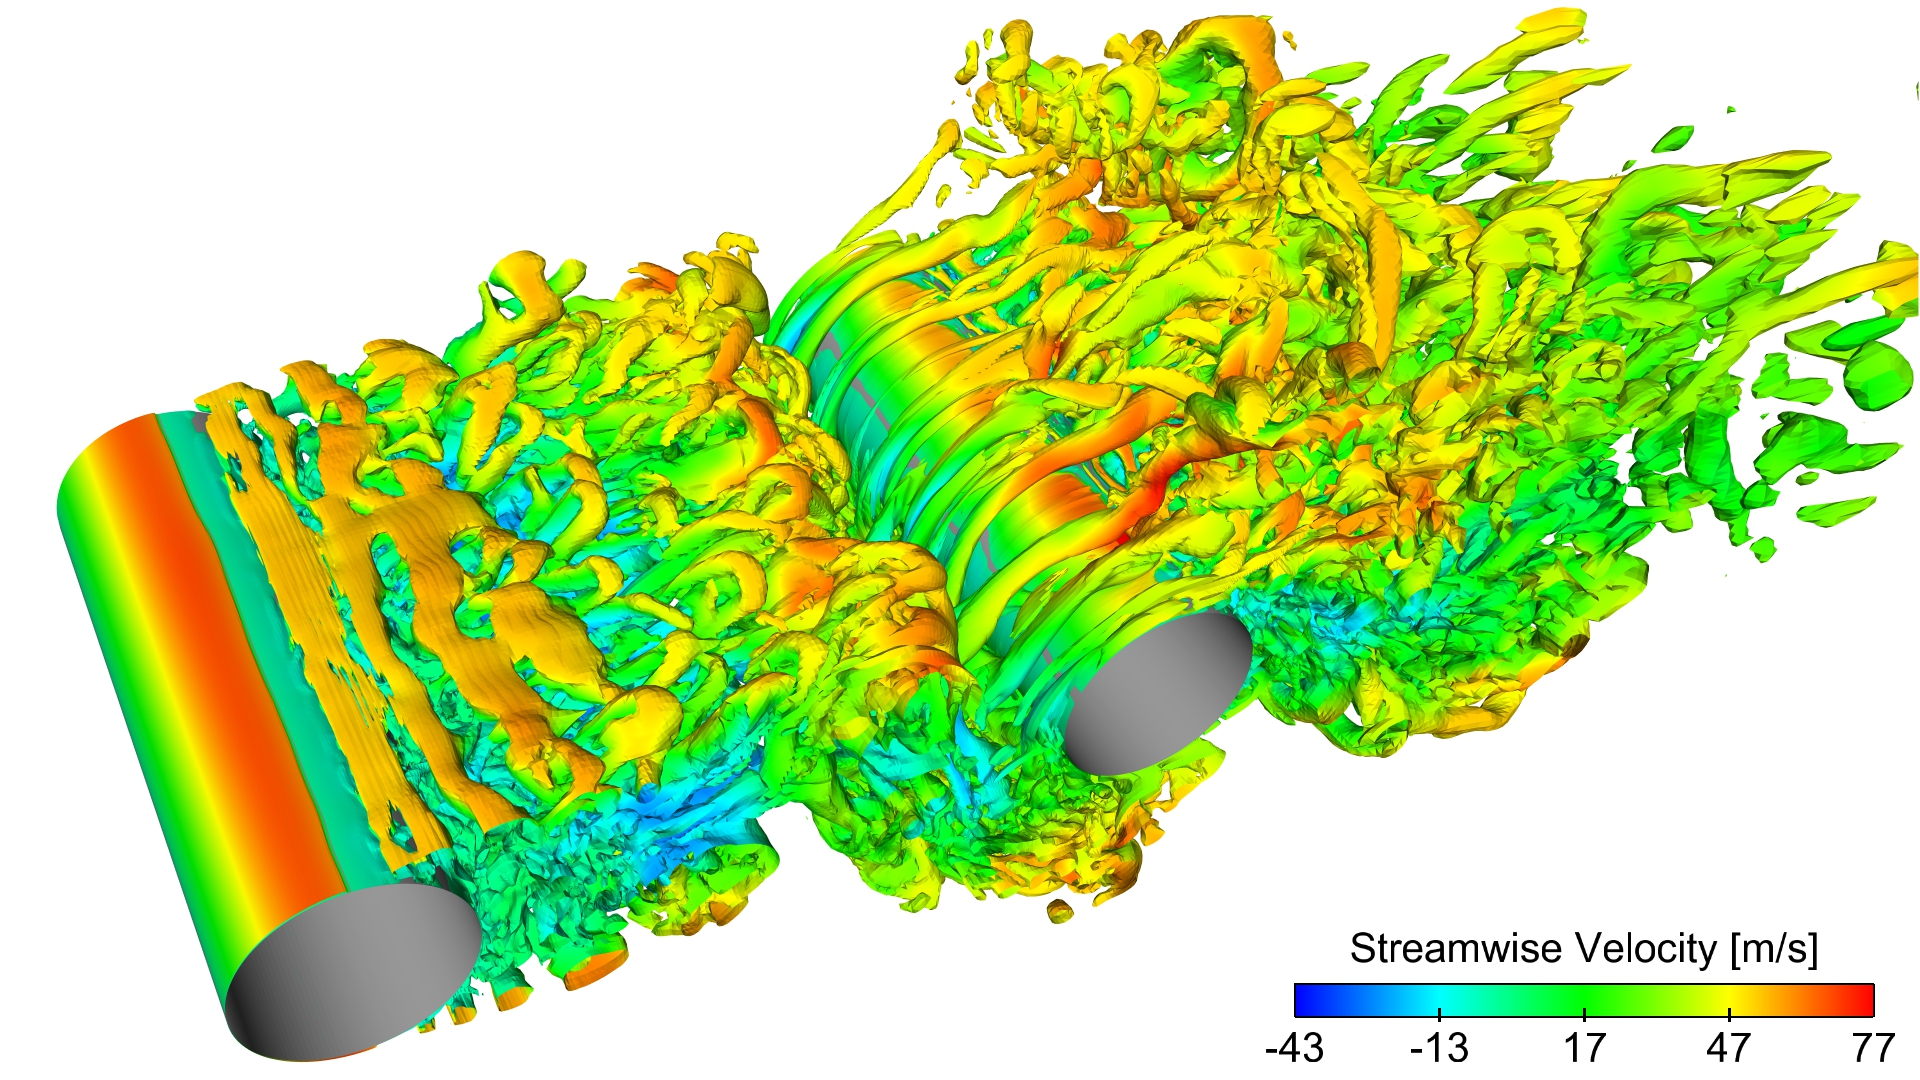
\includegraphics[width=0.40\textwidth]{tc_q_criteria}
    \caption[Q判据等值面图]{Q判据等值面图,同时测试一下一个很长的标题,比如这真的是一个很长很长很长很长很长很长很长很长的标题。}
    \label{fig:tc_q_criteria}
\end{figure}

若插图的空白区域过大,以图片\verb|shock_cyn|为例,自动裁剪如图
\ref{fig:shock_cyn}。
\begin{figure}[!htbp]
    \centering
    % trim option's parameter order: left bottom right top
    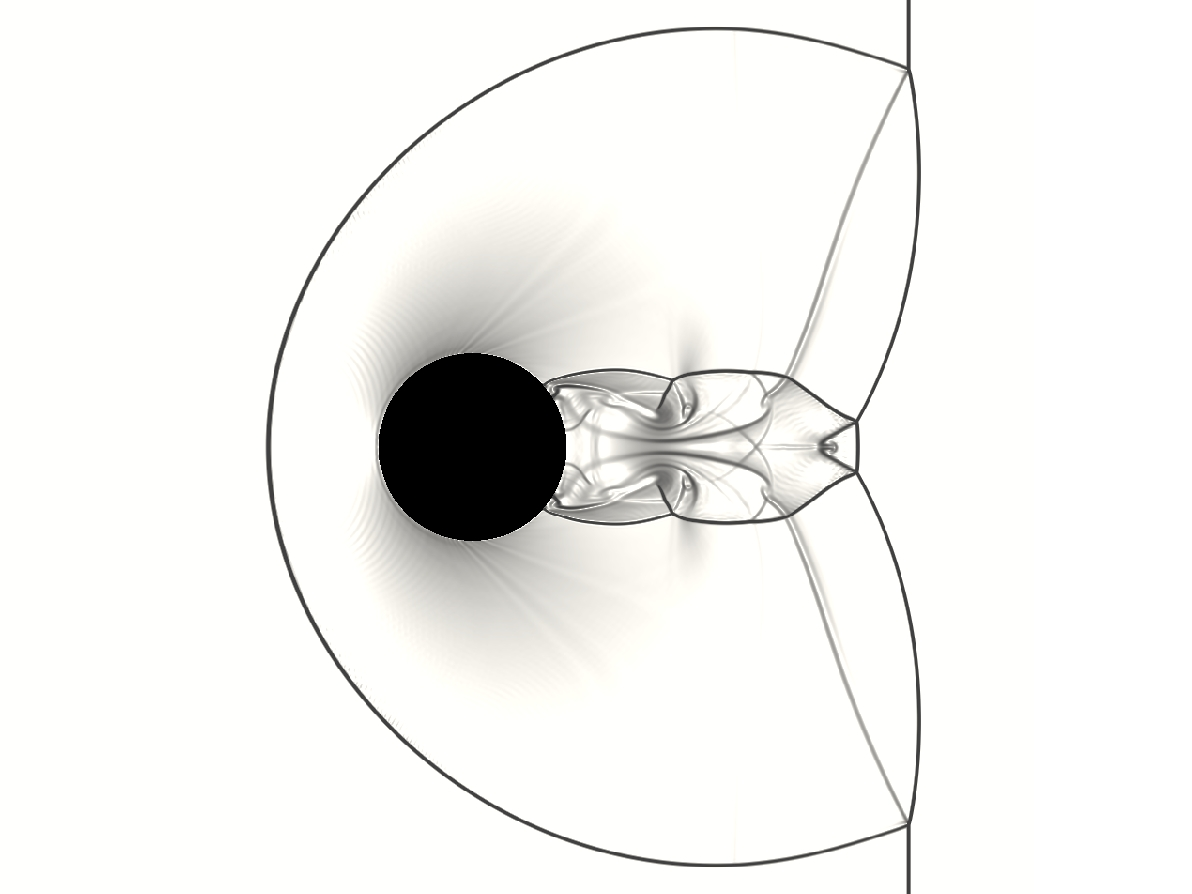
\includegraphics[trim = 30mm 0mm 30mm 0mm, clip, width=0.40\textwidth]{shock_cyn}
    \caption[激波圆柱作用]{激波圆柱作用。}
    \label{fig:shock_cyn}
\end{figure}

多图的插入如图~\ref{fig:oaspl},多图不应在子图中给文本子标题,只要给序号,并在主
标题中进行引用说明。
\begin{figure}[!htbp]
    \centering
    \begin{subfigure}[b]{0.35\textwidth}
      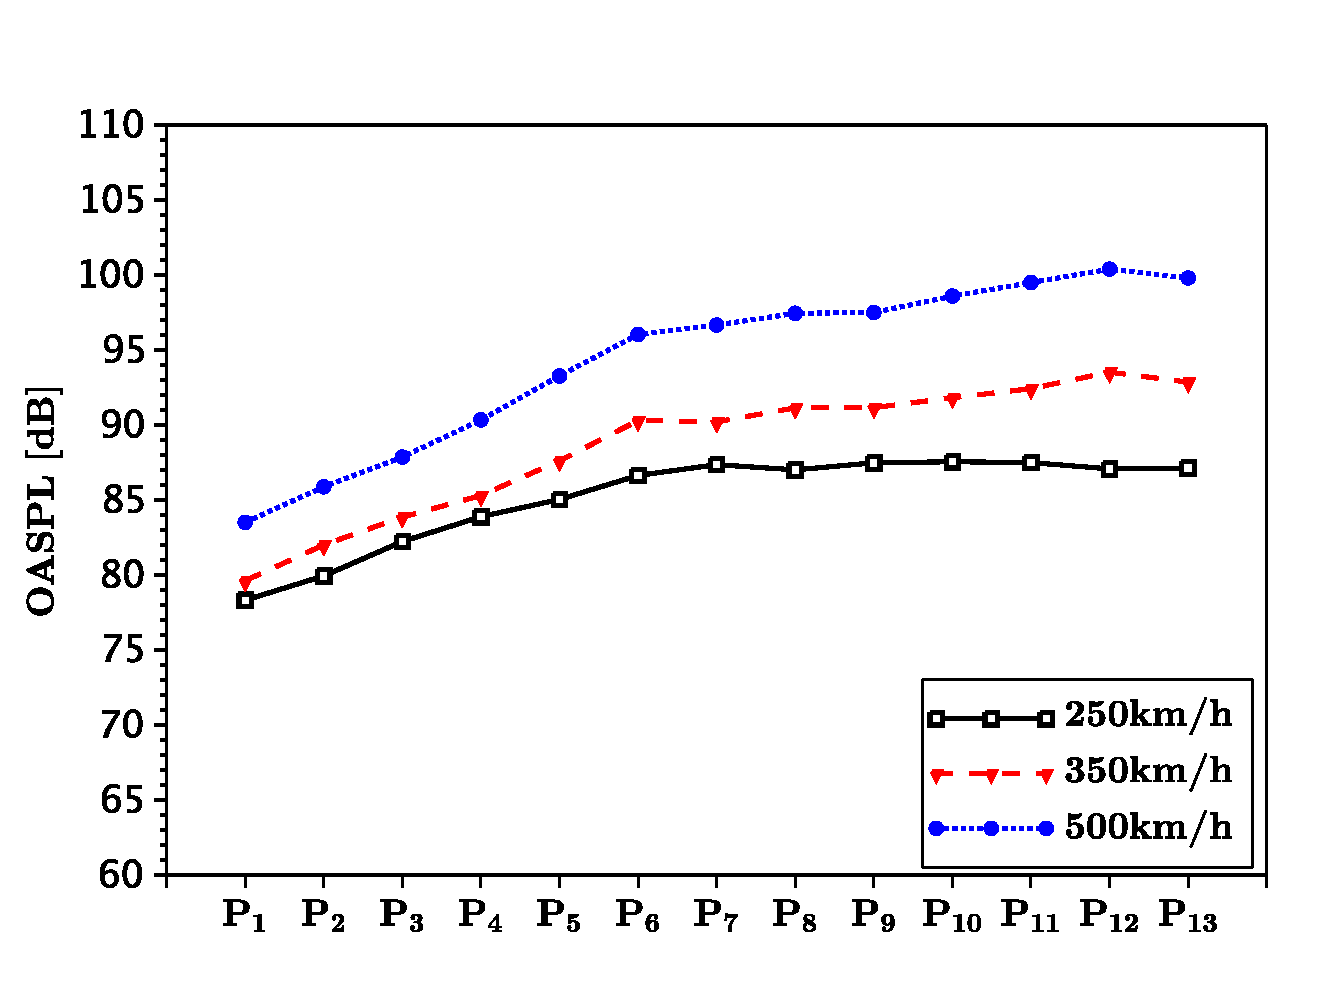
\includegraphics[width=\textwidth]{oaspl_a}
      \caption{}
      \label{fig:oaspl_a}
    \end{subfigure}%
    ~% add desired spacing
    \begin{subfigure}[b]{0.35\textwidth}
      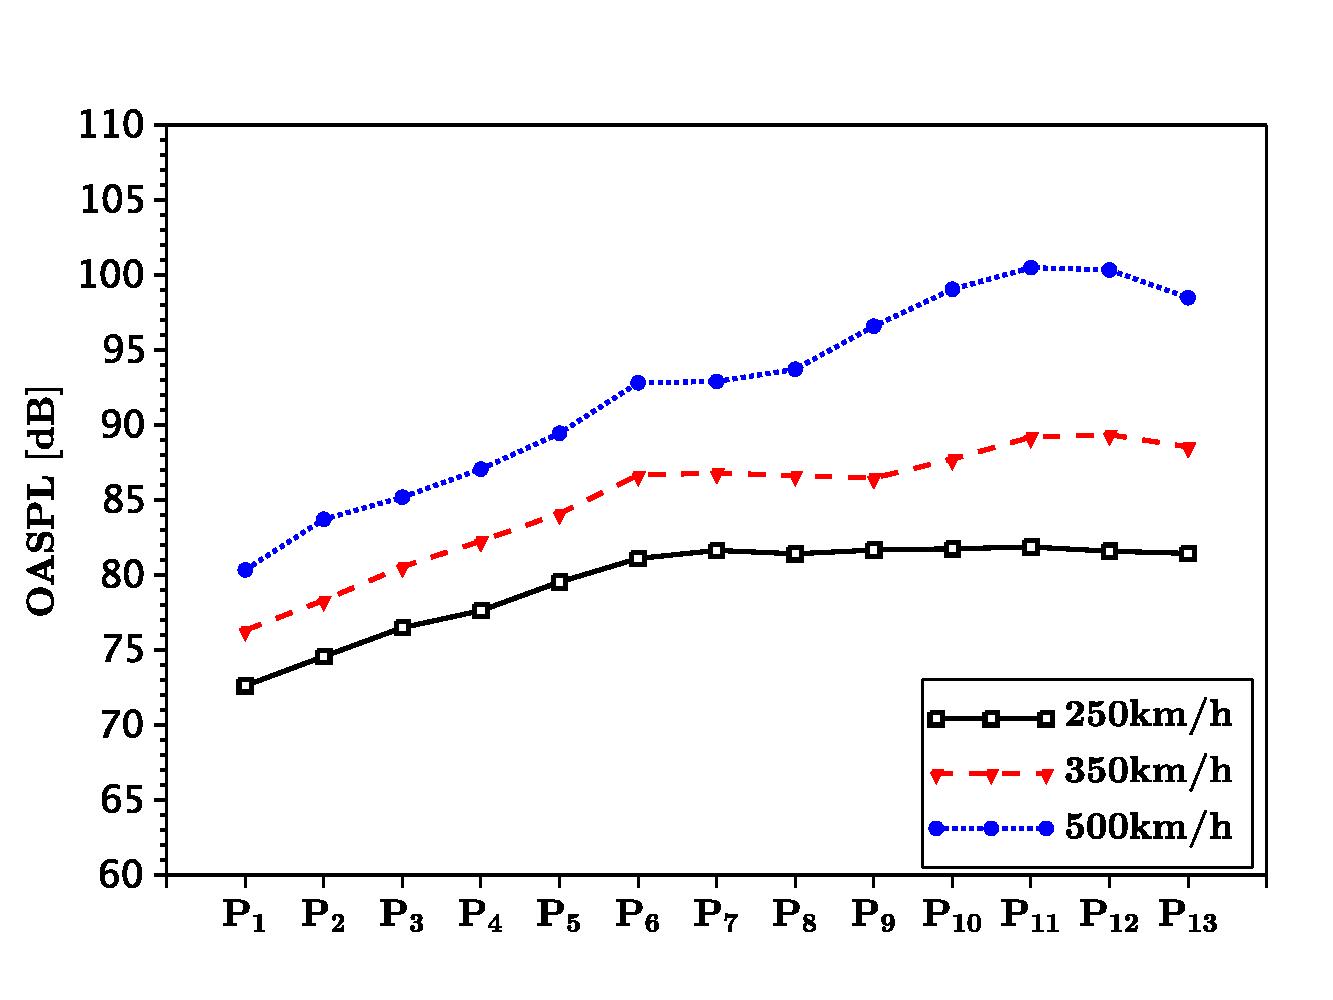
\includegraphics[width=\textwidth]{oaspl_b}
      \caption{}
      \label{fig:oaspl_b}
    \end{subfigure}
    \begin{subfigure}[b]{0.35\textwidth}
      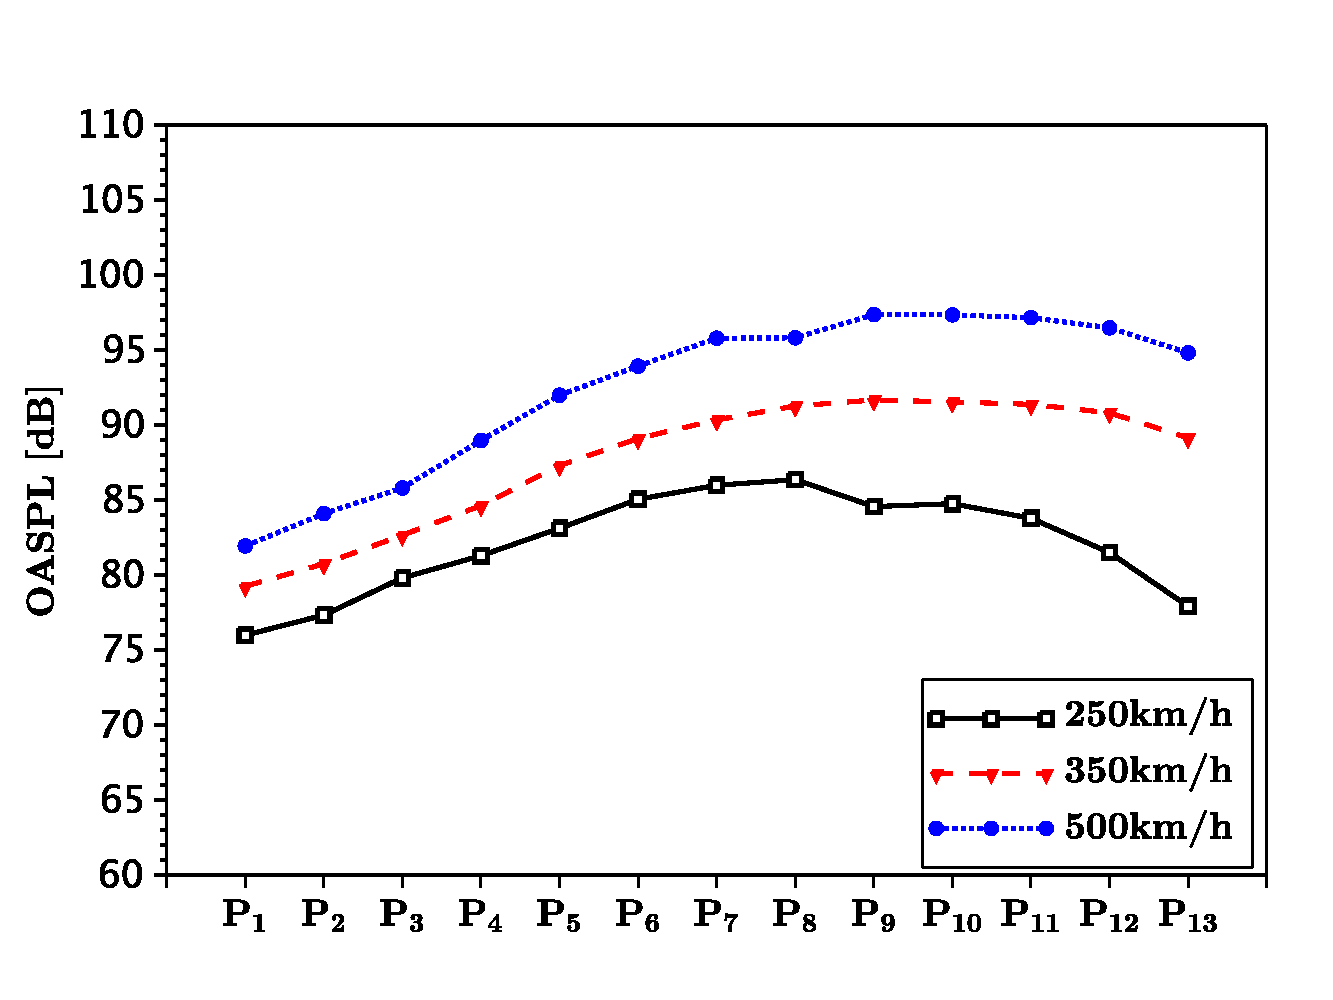
\includegraphics[width=\textwidth]{oaspl_c}
      \caption{}
      \label{fig:oaspl_c}
    \end{subfigure}%
    ~% add desired spacing
    \begin{subfigure}[b]{0.35\textwidth}
      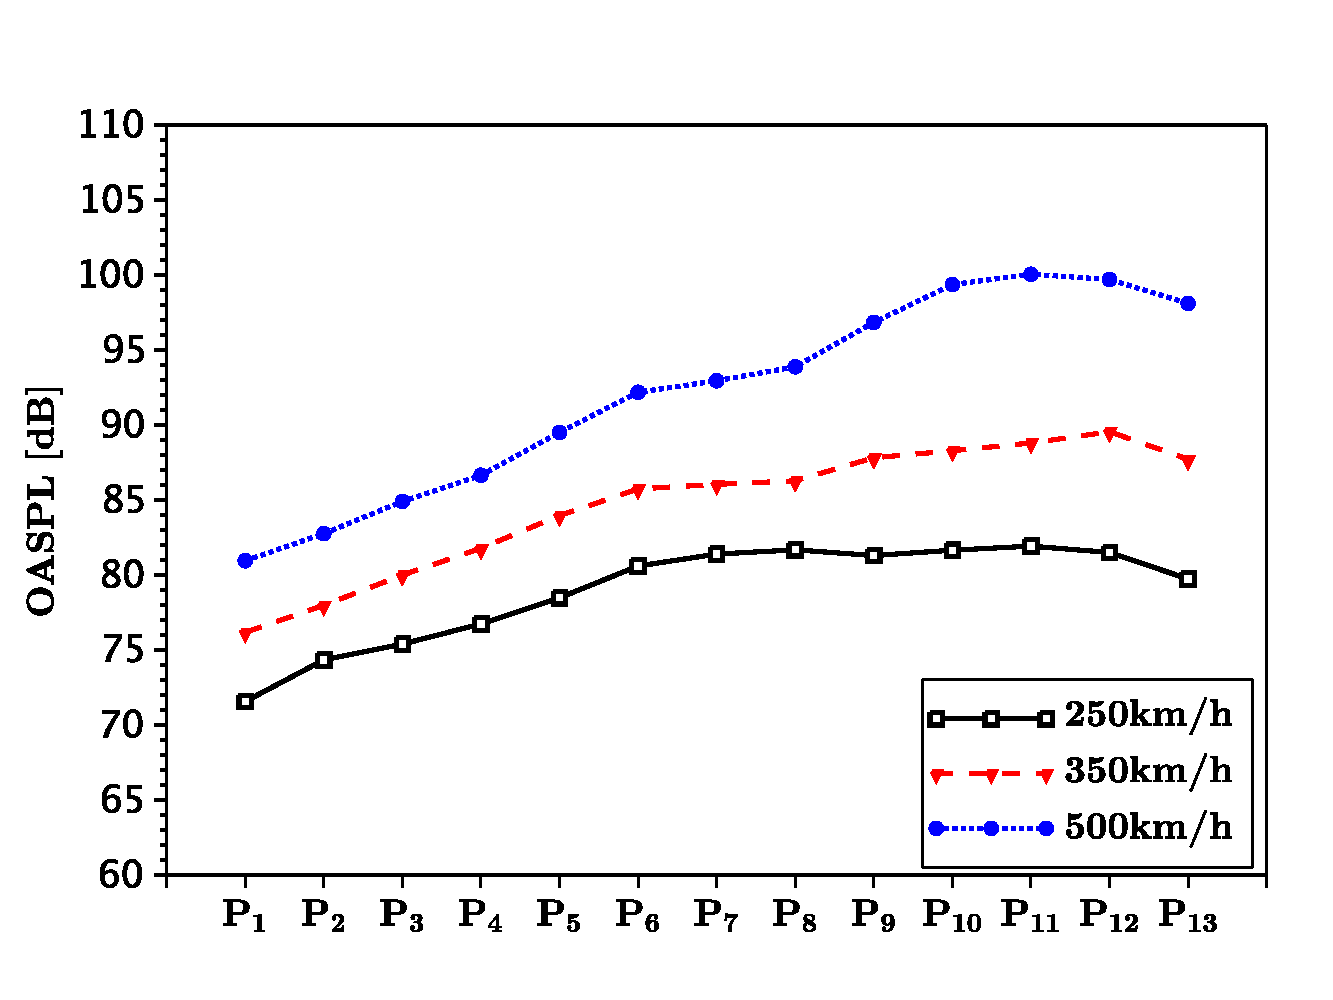
\includegraphics[width=\textwidth]{oaspl_d}
      \caption{}
      \label{fig:oaspl_d}
    \end{subfigure}
    \caption[总声压级]{总声压级。(a) 这是子图说明信息,(b) 这是子图说明信息,(c) 这是子图说明信息,(d) 这是子图说明信息。}
    \label{fig:oaspl}
\end{figure}

\subsection{算法}

算法环境在浙传毕设论文官方Word模板中未作明确要求,故暂采用通用样式,如算法
\ref{alg:euclid}所示,详细使用方法请参见文档
\href{https://ctan.org/pkg/algorithmicx?lang=en}{algorithmicx}。

\begin{algorithm}[!htbp]
    \small
    \caption{Euclid算法}\label{alg:euclid}
    \begin{algorithmic}[1]
        \Procedure{Euclid}{$a,b$}\Comment{$a$与$b$的最大公约数}
        \State $r\gets a\bmod b$
        \While{$r\not=0$}\Comment{若$r$为0则可跳出循环并返回答案}
        \State $a\gets b$
        \State $b\gets r$
        \State $r\gets a\bmod b$
        \EndWhile\label{euclidendwhile}
        \State \textbf{return} $b$\Comment{最大公约数为$b$}
        \EndProcedure
    \end{algorithmic}
\end{algorithm}

\subsection{代码段}

原则上,论文正文中应尽可能少的出现工程代码片段,建议每次不超过一页,并在正文中应
配有相应解释。这也体现了作者代码设计上的水平,即用尽可能少的代码完成尽可能具体的
任务。若必须引用一小段代码,可使用lstlisting设置代码环境。本模板的代码环境默认配
置在artratex.sty,搜索关键字“\verb|\lstset|”即可找到相应配置。

观察\autoref{code:samp-code},结合前述图表设置,试图理解代码环境的编写。

\begin{lstlisting}[
    language=c++,
    numbers=left,
    numberstyle=\tiny,
    label=code:samp-code,
    caption=一段Chromium的源代码
]
// Start tasks to take all the threads and block them.
const int kNumBlockTasks = static_cast<int>(kNumWorkerThreads);
for (int i = 0; i < kNumBlockTasks; ++i) {
    EXPECT_TRUE(pool()->PostWorkerTask(
        FROM_HERE,
        base::Bind(&TestTracker::BlockTask, tracker(), i, &blocker)));
}
tracker()->WaitUntilTasksBlocked(kNumWorkerThreads);

// Setup to open the floodgates from within Shutdown().
SetWillWaitForShutdownCallback(
    base::Bind(&TestTracker::PostBlockingTaskThenUnblockThreads,
                scoped_refptr<TestTracker>(tracker()), pool(), &blocker,
                kNumWorkerThreads));
pool()->Shutdown(kNumWorkerThreads + 1);

// Ensure that the correct number of tasks actually got run.
tracker()->WaitUntilTasksComplete(static_cast<size_t>(kNumWorkerThreads + 1));
tracker()->ClearCompleteSequence();
\end{lstlisting}

引用一两行代码,可以直接使用\texttt{verbatim}环境完成;若想调整环境中字体大小,
可先用\verb|\begingroup|和\verb|\endgroup|将其包住,后加入字体大小命令。注意,此
环境不会采取任何主动断行策略。

\begingroup
    \small
    \begin{verbatim}
Error: Command failed: /bin/sh -c rsync -arvq --exclude cache
--exclude .git 
    \end{verbatim}
\endgroup

\subsection{参考文献引用}

参考文献引用过程以实例进行介绍,假设需要引用名为``Document Preparation System''
的文献,步骤如下:
\begin{enumerate}
    \item 使用Google Scholar搜索Document Preparation System,在目标条目下点击
    Cite,展开后选择Import into BibTeX打开此文章的\hologo{BibTeX}索引信息,将它
    们copy添加到references.bib文件中(此文件位于bibliography文件夹下)。
    \item 索引第一行 \verb|@article{lamport1986document,|中
    \verb|lamport1986document|即为此文献的label (\textbf{中文文献也必须使用英文
    label},一般遵照:姓氏拼音+年份+标题第一字拼音的格式),想要在论文中索引此文
    献,有两种索引类型:
    \begin{itemize}
        \item 文本类型:\verb|\citet{lamport1986document}|,正如此处所示
        \citet{lamport1986document}; 
        \item 括号类型:\verb|\citep{lamport1986document}|。正如此处所示
        \citep{lamport1986document}。
    \end{itemize}
    \textbf{多文献索引用须用英文逗号隔开}:
    \begin{itemize}
        \item \verb|\citep{lamport1986document, chu2004tushu, chen2005zhulu}|,
        正如此处所示\citep{lamport1986document, chu2004tushu, chen2005zhulu}。
    \end{itemize}
\end{enumerate}

更多例子如:\citet{walls2013drought}根据...的研究,首次提出...。其中关于
...\citep{walls2013drought},是当前中国...得到迅速发展的研究领域
\citep{chen1980zhongguo}。引用同一著者在同一年份出版的多篇文献时,在出版年份之后
用英文小写字母区别,如:\citep{yuan2012lana, yuan2012lanb, yuan2012lanc}。同一处
引用多篇文献时,按出版年份由近及远依次标注,中间用分号分开,例如
\citep{chen1980zhongguo, stamerjohanns2009mathml, hls2012jinji, niu2013zonghe}。

使用著者-出版年制(authoryear)式参考文献样式时,中文文献必须在\hologo{BibTeX}索
引信息的\textbf{key} 域(请参考references.bib文件)填写作者姓名的拼音,才能使得
文献列表按照拼音排序。参考文献表中的条目(不排序号),先按语种分类排列,语种顺
序是:中文、日文、英文、俄文、其他文种。然后,中文按汉语拼音字母顺序排列,日文按
第一著者的姓氏笔画排序,西文和 俄文按第一著者姓氏首字母顺序排列。如中
\citep{niu2013zonghe}、日\citep{Bohan1928}、英\citep{stamerjohanns2009mathml}、
俄\citep{Dubrovin1906}。

不同文献样式和引用样式,如著者-出版年制(authoryear)、顺序编码制(numbers)、上
标顺序编码制(super)可在cuzthesis.tex中修改调用artratex.sty的参数实现,如:
\begin{itemize}
    \item \verb+\usepackage[numbers]{artratex}+ $\%$ 文本: Jones [1]; 括号: [1]
    \item \verb+\usepackage[super]{artratex}+ $\%$ 文本: Jones 上标[1]; 括号: 上标[1]
    \item \verb+\usepackage[authoryear]{artratex}+ $\%$ 文本: Jones (1995); 括号: (Jones, 1995)
    \item \verb+\usepackage[alpha]{artratex}+ $\%$ 文本: 不可用; 括号: [Jon95]
\end{itemize}

当前文档的默认参考文献样式为\textbf{super}。在该模式下,若希望在特定位置将上标改
为嵌入式标,可使用

\begin{itemize}
    \item 文本类型:\verb|\citetns{lamport1986document,chen2005zhulu}|,正如此处
    所示\citetns{lamport1986document,chen2005zhulu};
    \item 括号类型:\verb|\citepns{lamport1986document,chen2005zhulu}|;正如此处
    所示\citepns{lamport1986document,chen2005zhulu}。
\end{itemize}

参考文献索引更为详细的信息,请见
\href{https://github.com/zepinglee/gbt7714-bibtex-style}{zepinglee} 和
\href{https://en.wikibooks.org/wiki/LaTeX/Bibliography_Management}{WiKibook
Bibliography}。

\nocite{*}

\section{常见使用问题}\label{sec:qa}

\begin{enumerate}
    \item 模板每次发布前,都已在Windows,Linux,macOS系统上测试通过。下载模板
    后,若编译出现错误,则请参考国科大模板附带的
    \href{https://github.com/mohuangrui/ucasthesis/wiki}{\LaTeX{}知识小站} 中的
    \href{https://github.com/mohuangrui/ucasthesis/wiki/%E7%BC%96%E8%AF%91%E6%8C%87%E5%8D%97}{编
    译指南}。
    \item 模板文档的编码为UTF-8编码。所有文件都必须采用UTF-8编码,否则编译后生成
    的文档将出现乱码文本。若出现文本编辑器无法打开文档或打开文档乱码的问题,请检
    查编辑器对UTF-8编码的支持。
    \item 推荐选择\hologo{XeLaTeX}编译引擎编译中文文档。编译脚本的默认设定为
    \hologo{XeLaTeX}编译引擎。你也可以选择不使用脚本编译,如直接使用\LaTeX{}文本
    编辑器编译。注:\LaTeX{}文本编辑器编译的默认设定为\hologo{pdfLaTeX}编译引
    擎,若选择\hologo{XeLaTeX}编译引擎,请进入下拉菜单选择。为正确生成引用链接,
    需要进行全编译。由于\hologo{LuaLaTeX}编译引擎尚不成熟,故暂不推荐。
    \item vscode中关于\hologo{LaTeX}方面建议安装的插件:
        \begin{itemize}
            \item \hologo{LaTeX} Workshop:提供了绝大多数\hologo{LaTeX}的辅助功
            能;
            \item Rewrap:可使用\verb|Alt+Q|进行硬换行(即自动重排段落使得每行不
            超过指定宽度)。
        \end{itemize}
        其他一些有用的插件有:
        \begin{itemize}
            \item GitLens:提供了绝大多数Git的辅助功能;
            \item gitignore:对.gitignore文件进行操作;
            \item Markdown All in One:提供了Markdown语法支持与预览;
            \item Settings Sync:在不同平台间同步vscode插件及配置信息。
        \end{itemize}
    \item 设置文档样式: 在artratex.sty中搜索关键字定位相应命令,然后修改:
        \begin{itemize}
            \item 正文行距:启用和设置 \verb|\linespread{1.5}|,默认1.5倍行距。
            \item 参考文献行距:修改 \verb|\setlength{\bibsep}{0.0ex}|
            \item 目录显示级数:修改 \verb|\setcounter{tocdepth}{2}|
            \item 文档超链接的颜色及其显示:修改 \verb|\hypersetup|
        \end{itemize}
    \item 文档内字体切换方法:
        \begin{itemize}
            \item 宋体:浙传论文模板cuzthesis 或 \textrm{浙传论文模板cuzthesis}
            \item 粗宋体:{\bfseries 浙传论文模板cuzthesis} 或 \textbf{浙传论文模板cuzthesis}
            \item 黑体:{\sffamily 浙传论文模板cuzthesis} 或 \textsf{浙传论文模板cuzthesis}
            \item 粗黑体:{\bfseries\sffamily 浙传论文模板cuzthesis} 或 \textsf{\bfseries 浙传论文模板cuzthesis}
            \item 仿宋:{\ttfamily 浙传论文模板cuzthesis} 或 \texttt{浙传论文模板cuzthesis}
            \item 粗仿宋:{\bfseries\ttfamily 浙传论文模板cuzthesis} 或 \texttt{\bfseries 浙传论文模板cuzthesis}
            \item 楷体:{\itshape 浙传论文模板cuzthesis} 或 \textit{浙传论文模板cuzthesis}
            \item 粗楷体:{\bfseries\itshape 浙传论文模板cuzthesis} 或 \textit{\bfseries 浙传论文模板cuzthesis}
        \end{itemize}
\end{enumerate}


